\documentclass[tikz,border=12pt]{standalone}
\usepackage{amsmath,amssymb}
\usepackage{tikz}
\usetikzlibrary{arrows.meta,positioning,fit,calc,decorations.pathreplacing}

\definecolor{qtC}{HTML}{1F4E79}
\definecolor{stepC}{HTML}{B45309}
\definecolor{ink}{HTML}{1A1A1A}
\definecolor{bgSoft}{HTML}{F7F5F1}
\definecolor{gridC}{HTML}{9CA3AF}

\begin{document}
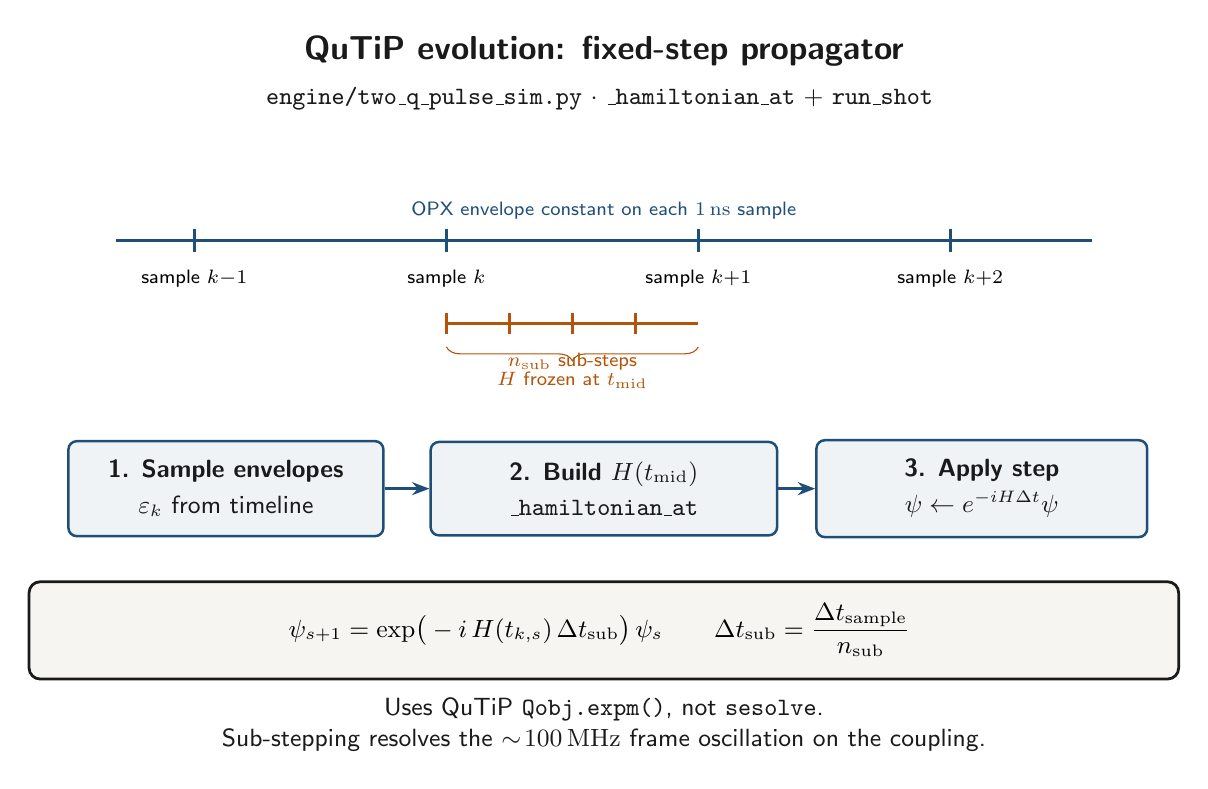
\begin{tikzpicture}[
  font=\sffamily\small,
  >={Stealth[length=2.2mm]},
  box/.style={
    draw=qtC, line width=0.9pt, rounded corners=3pt,
    fill=qtC!7, align=center, inner sep=7pt, text=ink
  },
  title/.style={font=\sffamily\bfseries\large, text=ink}
]

\node[title] at (0,5.0) {QuTiP evolution: fixed-step propagator};
\node[align=center, text=ink] at (0,4.4) {%
  \texttt{engine/two\_q\_pulse\_sim.py} $\cdot$
  \texttt{\_hamiltonian\_at} + \texttt{run\_shot}
};

% timeline schematic
\draw[line width=1.1pt, qtC] (-6.2,2.6) -- (6.2,2.6);
\foreach \x/\lab in {-5.2/k{-}1, -2.0/k, 1.2/{k{+}1}, 4.4/{k{+}2}} {
  \draw[line width=1pt, qtC] (\x,2.45) -- (\x,2.75);
  \node[below, font=\sffamily\scriptsize] at (\x,2.35) {sample $\lab$};
}
\node[above, font=\sffamily\scriptsize, text=qtC] at (0,2.75) {OPX envelope constant on each $1\,\mathrm{ns}$ sample};

% substeps inside sample k
\draw[line width=1.2pt, stepC] (-2.0,1.55) -- (1.2,1.55);
\foreach \i in {0,...,3} {
  \pgfmathsetmacro{\xx}{-2.0 + \i*0.8}
  \draw[line width=0.9pt, stepC] (\xx,1.42) -- (\xx,1.68);
}
\node[font=\sffamily\scriptsize, text=stepC, align=center] at (-0.4,0.95) {%
  $n_{\mathrm{sub}}$ sub-steps\\[-1pt]
  $H$ frozen at $t_{\mathrm{mid}}$
};

\draw[decorate, decoration={brace, amplitude=5pt, mirror}, stepC]
  (-2.0,1.25) -- (1.2,1.25);

% algorithm boxes
\node[box, minimum width=4.0cm] (B1) at (-4.8,-0.55) {%
  \textbf{1. Sample envelopes}\\[2pt]
  $\varepsilon_k$ from timeline
};

\node[box, minimum width=4.4cm] (B2) at (0,-0.55) {%
  \textbf{2. Build $H(t_{\mathrm{mid}})$}\\[2pt]
  \texttt{\_hamiltonian\_at}
};

\node[box, minimum width=4.2cm] (B3) at (4.8,-0.55) {%
  \textbf{3. Apply step}\\[2pt]
  $\psi\leftarrow e^{-iH\Delta t}\psi$
};

\draw[->, line width=1pt, qtC] (B1) -- (B2);
\draw[->, line width=1pt, qtC] (B2) -- (B3);

\node[draw=ink, line width=1pt, rounded corners=4pt, fill=bgSoft,
      align=center, inner sep=8pt, minimum width=14.6cm]
  (EQ) at (0,-2.35) {%
  $\displaystyle
  \psi_{s+1}
  =
  \exp\!\big(-i\,H(t_{k,s})\,\Delta t_{\mathrm{sub}}\big)\,\psi_s
  \qquad
  \Delta t_{\mathrm{sub}}=\frac{\Delta t_{\mathrm{sample}}}{n_{\mathrm{sub}}}$
};

\node[align=center, text=ink] at (0,-3.55) {%
  Uses QuTiP \texttt{Qobj.expm()}, not \texttt{sesolve}.\\
  Sub-stepping resolves the $\sim\!100\,\mathrm{MHz}$ frame oscillation on the coupling.
};

\end{tikzpicture}
\end{document}
